\documentclass[12pt,a4paper,fleqn]{narms}

% packages needed
\usepackage{subfigure}
\usepackage{epsfig}
\usepackage{timesmt}

% add here more packages based on the document format

\usepackage[utf8]{inputenc}
\usepackage[OT1]{fontenc}
\usepackage{graphicx}
\usepackage[english]{babel}

\usepackage{amsmath}
\usepackage{amsfonts}
\usepackage{amssymb}
\usepackage{amsthm}
\usepackage{bm}

\usepackage[usenames,dvipsnames]{xcolor}
\usepackage{url}
\usepackage{tikz}

\usepackage[bookmarks]{hyperref}

\usepackage{chicaco}

% setting math equation indent from left 0pts

%\mathindent=0pt%

\newcommand{\reals}{\mathbb{R}}
\newcommand{\posreals}{\reals_{>0}}
\newcommand{\posrealszero}{\reals_{\ge 0}}
\newcommand{\naturals}{\mathbb{N}}

\newcommand{\dd}{\,\mathrm{d}}

\newcommand{\mbf}[1]{\mathbf{#1}}
\newcommand{\bs}[1]{\boldsymbol{#1}}
\renewcommand{\vec}[1]{{\bm#1}}

\newcommand{\uz}{^{(0)}} % upper zero
\newcommand{\un}{^{(n)}} % upper n
\newcommand{\ui}{^{(i)}} % upper i

\newcommand{\ul}[1]{\underline{#1}}
\newcommand{\ol}[1]{\overline{#1}}

\newcommand{\Rsys}{R_\text{sys}}
\newcommand{\lRsys}{\ul{R}_\text{sys}}
\newcommand{\uRsys}{\ol{R}_\text{sys}}

\newcommand{\Fsys}{F_\text{sys}}
\newcommand{\lFsys}{\ul{F}_\text{sys}}
\newcommand{\uFsys}{\ol{F}_\text{sys}}

\def\Tsys{T_\text{sys}}

\newcommand{\E}{\operatorname{E}}
\newcommand{\V}{\operatorname{Var}}
\newcommand{\wei}{\operatorname{Wei}} % Weibull Distribution
\newcommand{\ig}{\operatorname{IG}}   % Inverse Gamma Distribution

\def\yz{y\uz}
\def\yn{y\un}
%\def\yi{y\ui}
\newcommand{\yfun}[1]{y^{({#1})}}
\newcommand{\yfunl}[1]{\ul{y}^{({#1})}}
\newcommand{\yfunu}[1]{\ol{y}^{({#1})}}

\def\ykz{y\uz_k}
\def\ykn{y\un_k}

\def\yzl{\ul{y}\uz}
\def\yzu{\ol{y}\uz}
\def\ynl{\ul{y}\un}
\def\ynu{\ol{y}\un}
\def\yil{\ul{y}\ui}
\def\yiu{\ol{y}\ui}

\def\ykzl{\ul{y}\uz_k}
\def\ykzu{\ol{y}\uz_k}
\def\yknl{\ul{y}\un_k}
\def\yknu{\ol{y}\un_k}


\def\nz{n\uz}
\def\nn{n\un}
%\def\ni{n\ui}
\newcommand{\nfun}[1]{n^{({#1})}}
\newcommand{\nfunl}[1]{\ul{n}^{({#1})}}
\newcommand{\nfunu}[1]{\ol{n}^{({#1})}}

\def\nkz{n\uz_k}
\def\nkn{n\un_k}


\def\nzl{\ul{n}\uz}
\def\nzu{\ol{n}\uz}
\def\nnl{\ul{n}\un}
\def\nnu{\ol{n}\un}
\def\nil{\ul{n}\ui}
\def\niu{\ol{n}\ui}

\def\nkzl{\ul{n}\uz_k}
\def\nkzu{\ol{n}\uz_k}
\def\nknl{\ul{n}\un_k}
\def\nknu{\ol{n}\un_k}


\def\taut{\tau(\vec{t})}
\def\ttau{\tilde{\tau}}
\def\ttaut{\ttau(\vec{t})}

\def\MZ{\mathcal{M}\uz}
\def\MN{\mathcal{M}\un}

\def\MkZ{\mathcal{M}\uz_k}
\def\MkN{\mathcal{M}\un_k}

\def\PkZ{\Pi\uz_k}
\def\PkN{\Pi\un_k}

\def\tnow{t_\text{now}}
\def\tpnow{t^+_\text{now}}

\newcommand{\comments}[1]{{\small\color{gray} #1}}

\newtheorem{example}{Example}

\allowdisplaybreaks

\title{Notes for ISIPTA poster}
\author{Gero Walter, Frank P.A. Coolen, Simme Douwe Flapper}

\begin{document}
\maketitle

(Notation more similar to risk analysis paper.)

System with components of $k=1,\ldots,K$ different types.
There are $n_k$ components of type $k$ in the system.

For each $k$, component lifetimes ($i=1,\ldots,n_k$) are $T_i^k \mid \lambda_k \sim \wei(\kappa,\lambda_k)$,
where $\kappa$ is fixed and known:
\begin{align}
f_k(t_i^k \mid \lambda_k) &= \frac{\kappa}{\lambda_k} (t_i^k)^{\kappa-1} e^{-\frac{(t_i^k)^{\kappa-1}}{\lambda_k}} \\
F_k(t_i^k \mid \lambda_k) &= 1 - e^{-\frac{(t_i^k)^{\kappa-1}}{\lambda_k}} = P_k(T_i^k \leq t_i^k \mid \lambda_k)
\end{align}

Conjugate prior is $\lambda_k \sim \ig(\alpha_k,\beta_k)$:
\begin{align}
f_{\lambda_k}(\lambda_k\mid \alpha_k,\beta_k) &= \frac{(\beta_k)^{\alpha_k}}{\Gamma(\alpha_k)} \lambda_k^{-\alpha_k -1} e^{-\frac{\beta_k}{\lambda_k}}
\end{align}
In terms of canonical parameters $\nkz,\ykz$, $\lambda_k \mid \nkz,\ykz \sim \ig(\nkz + 1, \nkz\ykz)$.

Set of priors $\MkZ$ defined by $(\nkz,\ykz) \in \PkZ = [\nkzl,\nkzu] \times [\ykzl,\ykzu]$.

Observing a one of a kind system with $n_k$ components of type $k$ running until $\tnow$,
where $e_k$ components have failed by $\tnow$, and $n_k - e_k$ components still function:
\begin{align}
\mbf{t}^k_{e_k;n_k} &= \big( \underbrace{t^k_1, \ldots, t^k_{e_k}}_{e_k \text{failure times}},
                             \underbrace{\tpnow, \ldots, \tpnow}_{n_k-e_k \text{censored obs.}} \big)
\end{align}

Posterior:
\begin{align}
f_{\lambda_k\mid\ldots}(\lambda_k\mid\nkz,\ykz,\mbf{t}^k_{e_k;n_k})
 &\propto f_{\lambda_k}(\lambda_k)
          \big[ 1- F_k(\tnow\mid\lambda_k) \big]^{n_k-e_k}
          \prod_{i=1}^{e_k} f_k(t_i^k \mid \lambda_k) 
\end{align}
and so $\lambda_k\mid\nkz,\ykz,\mbf{t}^k_{e_k;n_k} \sim \ig(\nkn + 1, \nkn\ykn)$, where
\begin{align}
\nkn + 1 &= \nkz + e_k + 1 \\
\nkn\ykn &= \nkz\ykz + (n_k-e_k) \tnow^\kappa + \sum_{i=1}^{e_k} (t_i^k)^\kappa
\end{align}

\newpage

System survival calculated by (see Risk Analysis paper eq. (7))
\begin{align}
P(\Tsys > t) &= \sum_{l_1=1}^{n_1} \cdots \sum_{l_K=1}^{n_K} \Phi(l_1,\ldots,\l_K) P\Big( \bigcap_{k=1}^K \{ C^k_t = l_k\} \Big) \\
\intertext{ and assuming components of different types are independent,}
             &= \sum_{l_1=1}^{n_1} \cdots \sum_{l_K=1}^{n_K} \Phi(l_1,\ldots,\l_K) \prod_{k=1}^K P(C^k_t = l_k)
\end{align}
where the survival signature $\Phi(l_1,\ldots,\l_K)$ is non-decreasing in each $l_k$ for coherent systems,
and $P(C^k_t = l_k)$ is the (predictive) probability that exactly $l_k$ components of type $k$ function at time $t$.

A priori, we have, for $l_k = 0,1,\ldots, n_k$,
\begin{align}
P(C^k_t = l_k\mid\nkz,\ykz)
 &= { n_k \choose l_k} \int [F_k(t \mid\lambda_k)]^{n_k-l_k}
                        [1 - F_k(t \mid\lambda_k)]^{l_k} f_{\lambda_k}(\lambda_k\mid\nkz,\ykz) \dd \lambda_k
\end{align}
under the assumption that components of the same type are independent given $\lambda_k$.

\bigskip

For the situation with the system observed until $\tnow$, with data $\mbf{t}^k_{e_k;n_k}$,
we need the posterior predictive probability $P(C^k_t = l_k\mid\nkz,\ykz, \mbf{t}^k_{e_k;n_k})$.

For $l_k > n_k - e_k$, we must have $P(C^k_t = l_k\mid\nkz,\ykz, \mbf{t}^k_{e_k;n_k}) = 0$,
as at most $n_k - e_k$ components can function for $t > \tnow$.

(Should one work with the subsystem consisting only of the non-failed $n_k - e_k$ components?)\\

A posteriori, we have, for $l_k = 0,1,\ldots, n_k - e_k$,
\begin{align}
P(C^k_t = l_k\mid\nkz,\ykz, \mbf{t}^k_{e_k;n_k})
 &= { n_k - e_k \choose l_k} \int [P_k(T \leq t \mid T > \tnow, \lambda_k)]^{n_k - e_k - l_k} \times \\ & \hspace*{7ex}
                              [1 - P_k(T \leq t \mid T > \tnow, \lambda_k)]^{l_k}
    f_{\lambda_k\mid\ldots}(\lambda_k\mid\nkz,\ykz,\mbf{t}^k_{e_k;n_k}) \dd \lambda_k
\end{align}

Now,
\begin{align}
P_k(T \leq t \mid T > \tnow, \lambda_k)
 &= \frac{P_k(\tnow < T \leq t \mid\lambda_k)}{P_k(T > \tnow \mid \lambda_k)}
  = \frac{F_k(t\mid\lambda_k) - F_k(\tnow\mid\lambda_k)}{1-F_k(\tnow\mid\lambda_k)} \\
 &= \frac{e^{-\frac{(\tnow)^\kappa}{\lambda_k}} - e^{-\frac{t^\kappa}{\lambda_k}}}{e^{-\frac{(\tnow)^\kappa}{\lambda_k}}}
  = 1 - e^{-\frac{t^\kappa - (\tnow)^\kappa}{\lambda_k}}
\end{align}

With this and the posterior substituted in, we get
\begin{align}
\lefteqn{P(C^k_t = l_k\mid\nkz,\ykz, \mbf{t}^k_{e_k;n_k})} \\
 &= { n_k - e_k \choose l_k} \int \Big[1 - e^{-\frac{t^\kappa - (\tnow)^\kappa}{\lambda_k}}\Big]^{n_k - e_k - l_k}
                                  \Big[    e^{-\frac{t^\kappa - (\tnow)^\kappa}{\lambda_k}}\Big]^{l_k} %\times \\ & \hspace*{25ex}
    \frac{[\nkn\ykn]^{\nkn + 1}}{\Gamma(\nkn+1)} \lambda_k^{-(\nkn + 1) - 1} e^{-\frac{\nkn\ykn}{\lambda_k}} \dd \lambda_k \\
 &= { n_k - e_k \choose l_k} \sum_{j=0}^{n_k-e_k-l_k} (-1)^j { n_k - e_k - l_k \choose j} \frac{[\nkn\ykn]^{\nkn + 1}}{\Gamma(\nkn+1)} 
    \int \lambda_k^{-(\nkn + 1) - 1} e^{-\frac{(l_k + j) (t^\kappa - (\tnow)^\kappa) + \nkn\ykn}{\lambda_k}} \dd \lambda_k
\end{align}

The terms remaining under the integral form the core of an $\ig(\nkn + 1, \nkn\ykn + (l_k + j) (t^\kappa - (\tnow)^\kappa))$,
allowing us to solve the integral using the corresponding normalization constant.
\begin{align}
\lefteqn{P(C^k_t = l_k\mid\nkz,\ykz, \mbf{t}^k_{e_k;n_k})} \\
 &= { n_k - e_k \choose l_k} \sum_{j=0}^{n_k-e_k-l_k} (-1)^j { n_k - e_k - l_k \choose j}
    \left(\frac{\nkn\ykn}{\nkn\ykn + (l_k + j) (t^\kappa - (\tnow)^\kappa)}\right)^{\nkn + 1} \\
 &= \sum_{j=0}^{n_k-e_k-l_k} (-1)^j \frac{(n_k - e_k)!}{l_k! j! (n_k - e_k - l_k - j)!}   
    \left(\frac{\nkn\ykn}{\nkn\ykn + (l_k + j) (t^\kappa - (\tnow)^\kappa)}\right)^{\nkn + 1} \\
 &= \sum_{j=0}^{n_k-e_k-l_k} (-1)^j \frac{(n_k - e_k)!}{l_k! j! (n_k - e_k - l_k - j)!} \times \\ & \hspace*{20ex}  
    \left(\frac{\nkz\ykz + \sum_{i=1}^{e_k} (t_i^k)^\kappa + (n_k-e_k) (\tnow)^\kappa }%
               {\nkz\ykz + \sum_{i=1}^{e_k} (t_i^k)^\kappa + (n_k-e_k-l_k-j) (\tnow)^\kappa + (l_k + j) t^\kappa }\right)^{%
    \nkz + e_k + 1} 
\end{align}
for $l_k \in \{0,1,\ldots,n_k-e_k\}$.

(We actually need only those $P(C^k_t = l_k\mid \ldots)$ with $l_k$'s
for which $\Phi(l_1,\ldots,\l_K) > 0$!)


Seen as function in $t$, we see that $t$ appears $n_k-e_k-l_k+1$ times,
once in each summand, in the denominator of the fraction powered to the $\nkn+1$.
Nevertheless, $P(C^k_t = l_k\mid\nkz,\ykz, \mbf{t}^k_{e_k;n_k})$
must be decreasing in $t$, as the remaining $n_k-e_k$ components continue to age,
and so the probability that $l_k$ of them remain operational must decrease.

I would think that
$\min / \max_{(\nkz,\ykz) \in \PkZ} P(C^k_t = l_k\mid\nkz,\ykz, \mbf{t}^k_{e_k;n_k})$
must be solved by numeric optimization for each $k, l_k, t$ 
because of the alternating signs for the summands.
(In absolute terms, each summand is increasing in $\ykz$, but not monotone in $\nkz$.)

(Box-constraint optimization possible, e.g., with option \texttt{L-BFGS-B} of \texttt{optim} in \textbf{R}.)

Do I get your comments right that based on lower and upper bounds
$\ul{P}(C^k_t = l_k\mid \ldots)$ and $\ol{P}(C^k_t = l_k\mid \ldots)$ for all $l_k = 0, 1, \ldots, n_k - e_k$,
we can easily get lower and upper bounds for the cdf $F_{C^k_t}(l_k \mid \ldots)$?

The cdf for $C^k_t$ is 
\begin{align}
%F_{C^k_t}(l_k \mid \nkz,\ykz, \mbf{t}^k_{e_k;n_k}) = P(C^k_t \leq l_k\mid\nkz,\ykz, \mbf{t}^k_{e_k;n_k}) 
% = \sum_{q=0}^{l_k} P(C^k_t = q\mid\nkz,\ykz, \mbf{t}^k_{e_k;n_k})
F_{C^k_t}(l_k \mid \ldots) = P(C^k_t \leq l_k\mid\ldots) = \sum_{q=0}^{l_k} P(C^k_t = q\mid\ldots)
\end{align} 
But I don't see how $\ul{F}_{C^k_t}(l_k \mid \ldots)$ and $\ol{F}_{C^k_t}(l_k \mid \ldots)$
help us for the lower and upper system survival function,
the system survival for $t > \tnow$ being
\begin{align}
P(\Tsys > t\mid\nkz,\ykz, \mbf{t}^k_{e_k;n_k})
 &= \sum_{l_1=1}^{n_1-e_1} \cdots \sum_{l_K=1}^{n_K-e_K} \Phi(l_1,\ldots,\l_K) \prod_{k=1}^K
    P(C^k_t = l_k\mid\nkz,\ykz, \mbf{t}^k_{e_k;n_k}) \,.
\end{align}

We cannot simply plug in all the $\ul{P}(C^k_t = l_k\mid \ldots)$ %and $\ol{P}(C^k_t = l_k\mid \ldots)$
into the above to get $\ul{P}(\Tsys > t\mid\nkz,\ykz, \mbf{t}^k_{e_k;n_k})$, % and $\ol{P}(\Tsys > t\mid\nkz,\ykz, \mbf{t}^k_{e_k;n_k})$,
as the $\ul{P}(C^k_t = l_k\mid \ldots)$ could correspond to different $(\nkz,\ykz)$ for each $l_k$.
(It would give us a lower bound for $\ul{P}(\Tsys > t\mid\ldots)$, however, but it might be very coarse.)

So do we have to make the optimization over $(\nkz,\ykz)$ for the full expression below?

\begin{align}
\lefteqn{P(\Tsys > t\mid\nkz,\ykz, \mbf{t}^k_{e_k;n_k})} \\
 &= \sum_{l_1=1}^{n_1-e_1} \cdots \sum_{l_K=1}^{n_K-e_K} \Phi(l_1,\ldots,\l_K) \prod_{k=1}^K
    P(C^k_t = l_k\mid\nkz,\ykz, \mbf{t}^k_{e_k;n_k}) \\
 &= \sum_{l_1=1}^{n_1-e_1} \cdots \sum_{l_K=1}^{n_K-e_K} \Phi(l_1,\ldots,\l_K) \prod_{k=1}^K
    \sum_{j=0}^{n_k-e_k-l_k} (-1)^j \frac{(n_k - e_k)!}{l_k! j! (n_k - e_k - l_k - j)!} \times \\ & \hspace*{45ex}
    \left(\frac{\nkn\ykn}{\nkn\ykn + (l_k + j) (t^\kappa - (\tnow)^\kappa)}\right)^{\nkn + 1} \\
 &= \sum_{l_1=1}^{n_1-e_1} \cdots \sum_{l_K=1}^{n_K-e_K} \Phi(l_1,\ldots,\l_K) \prod_{k=1}^K
    \sum_{j=0}^{n_k-e_k-l_k} (-1)^j \frac{(n_k - e_k)!}{l_k! j! (n_k - e_k - l_k - j)!} \times \\ & \hspace*{17ex}
    \left(\frac{\nkz\ykz + \sum_{i=1}^{e_k} (t_i^k)^\kappa + (n_k-e_k) (\tnow)^\kappa }%
               {\nkz\ykz + \sum_{i=1}^{e_k} (t_i^k)^\kappa + (n_k-e_k-l_k-j) (\tnow)^\kappa + (l_k + j) t^\kappa }\right)^{%
    \nkz + e_k + 1} 
\end{align}


The example system with $k=3$ component types, $n_1=2$, $n_2=2$, $n_3=1$:

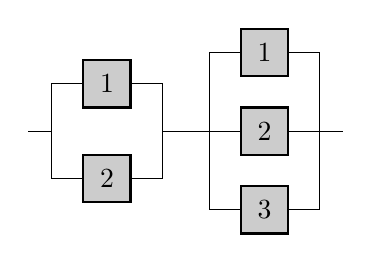
\begin{tikzpicture}
[type1/.style={rectangle,draw,fill=black!20,thick,inner sep=0pt,minimum size=6mm},
 type2/.style={rectangle,draw,fill=black!20,thick,inner sep=0pt,minimum size=6mm},
 type3/.style={rectangle,draw,fill=black!20,thick,inner sep=0pt,minimum size=6mm},
 hv path/.style={to path={-| (\tikztotarget)}},
 vh path/.style={to path={|- (\tikztotarget)}}]
\node[type1] (double1) at ( 1, 0.6) {1};
\node[type2] (double2) at ( 1,-0.6) {2};
\node[type1] (triple1) at ( 3, 1)  {1};
\node[type2] (triple2) at ( 3, 0)  {2};
\node[type3] (triple3) at ( 3,-1)  {3};
\coordinate (start) at (0,0);
\coordinate (bifst) at (0.3,0);
\coordinate (bifen) at (1.7,0);
\coordinate (trist) at (2.3,0);
\coordinate (trien) at (3.7,0);
\coordinate (end)   at (4,0);
\path (start) edge (bifst)
      (bifst) edge[vh path] (double1.west)
              edge[vh path] (double2.west)
      (bifen) edge[vh path] (double1.east)
              edge[vh path] (double2.east)
              edge (trist)
      (trist) edge[vh path] (triple1.west)
              edge          (triple2.west)
              edge[vh path] (triple3.west)
      (trien) edge[vh path] (triple1.east)
              edge          (triple2.east)
              edge[vh path] (triple3.east)
              edge          (end);
\end{tikzpicture}



\end{document}
